\documentclass[letterpaper,11pt]{article}
\oddsidemargin -1.0cm \textwidth 17.5cm

\usepackage[utf8]{inputenc}
\usepackage[activeacute,spanish, es-lcroman]{babel}
\decimalpoint
\usepackage{amsfonts,setspace}
\usepackage{amsmath}
\usepackage{amssymb, amsmath, amsthm}
\usepackage{comment}
\usepackage{float}
\usepackage{amssymb}
\usepackage{dsfont}
\usepackage{anysize}
\usepackage{multicol}
\usepackage{enumerate}
\usepackage{graphicx}
\usepackage[left=1.5cm,top=2cm,right=1.5cm, bottom=1.7cm]{geometry}
\setlength\headheight{1.5em} 
\usepackage{fancyhdr}
\usepackage{multicol}
\usepackage{hyperref}
\usepackage{wrapfig}
\usepackage{subcaption}
\usepackage{siunitx}
\usepackage{cancel}
\usepackage{mdwlist}
\usepackage{svg}
\pagestyle{fancy}
\fancyhf{}
\renewcommand{\labelenumi}{\normalsize\bfseries P\arabic{enumi}.}
\renewcommand{\labelenumii}{\normalsize\bfseries (\alph{enumii})}
\renewcommand{\labelenumiii}{\normalsize\bfseries \roman{enumiii})}


\begin{document}

\fancyhead[L]{\itshape{Facultad de Ciencias F\'isicas y Matem\'aticas}}
\fancyhead[R]{\itshape{Universidad de Chile}}

\begin{minipage}{11.5cm}
    \begin{flushleft}
        \hspace*{-0.6cm}\textbf{FI1000-1 Introducción a la Física Clásica}\\
        \hspace*{-0.6cm}\textbf{Profesor:} Ignacio Bordeu\\
        \hspace*{-0.6cm}\textbf{Auxiliares:} Javier Cubillos \& Berenice Muruaga\\
        \hspace*{-0.6cm}\textbf{Auxiliares taller:} Pablo González \& Alejandro Cartes\\
        \hspace*{-0.6cm}\textbf{Ayudante:} Amaru Moya\\
    \end{flushleft}
\end{minipage}

\begin{picture}(2,3)
    \put(366, 10){
\includegraphics[scale=0.9]{2020-1/Imágenes/logo/dfi-fcfm.pdf}}
\end{picture}

\begin{center}
	\LARGE\textbf{Taller \#6:}{\Large +dinámica}
\end{center}

\vspace{-1cm}
\begin{enumerate}\setlength{\itemsep}{0.4cm}

% \item[]
\vspace{2em}

\item
    \begin{enumerate}
        \item 
            Dado el sistema de la figura P1a, si el bloque de masa $M$ se mantiene en equilibrio gracias a la fuerza externa $F$ y a las cuerdas-poleas (ideales), determine el valor de la tensión en cada cuerda.
            
        \item Un bloque de masa $m_1$ se encuentra sobre una superficie horizontal (sin roce), y está unido a un bloque de masa $m_2$ a través de una polea móvil $P_1$ y una polea fija $P_2$ (ambas ideales), tal como se muestra en la figura P1b.
        
        \begin{enumerate}
            \item Demuestre que la aceleración de $m_1$ es el doble de la aceleración de $m_2$
            
            \item Determine la aceleración de cada bloque y la tensión en cada cuerda en función de $m_1$, $m_2$ y $g$
        \end{enumerate}
        
        \begin{figure}[H]
            \centering
            \begin{subfigure}[t]{0.4\linewidth} 
                \centering
                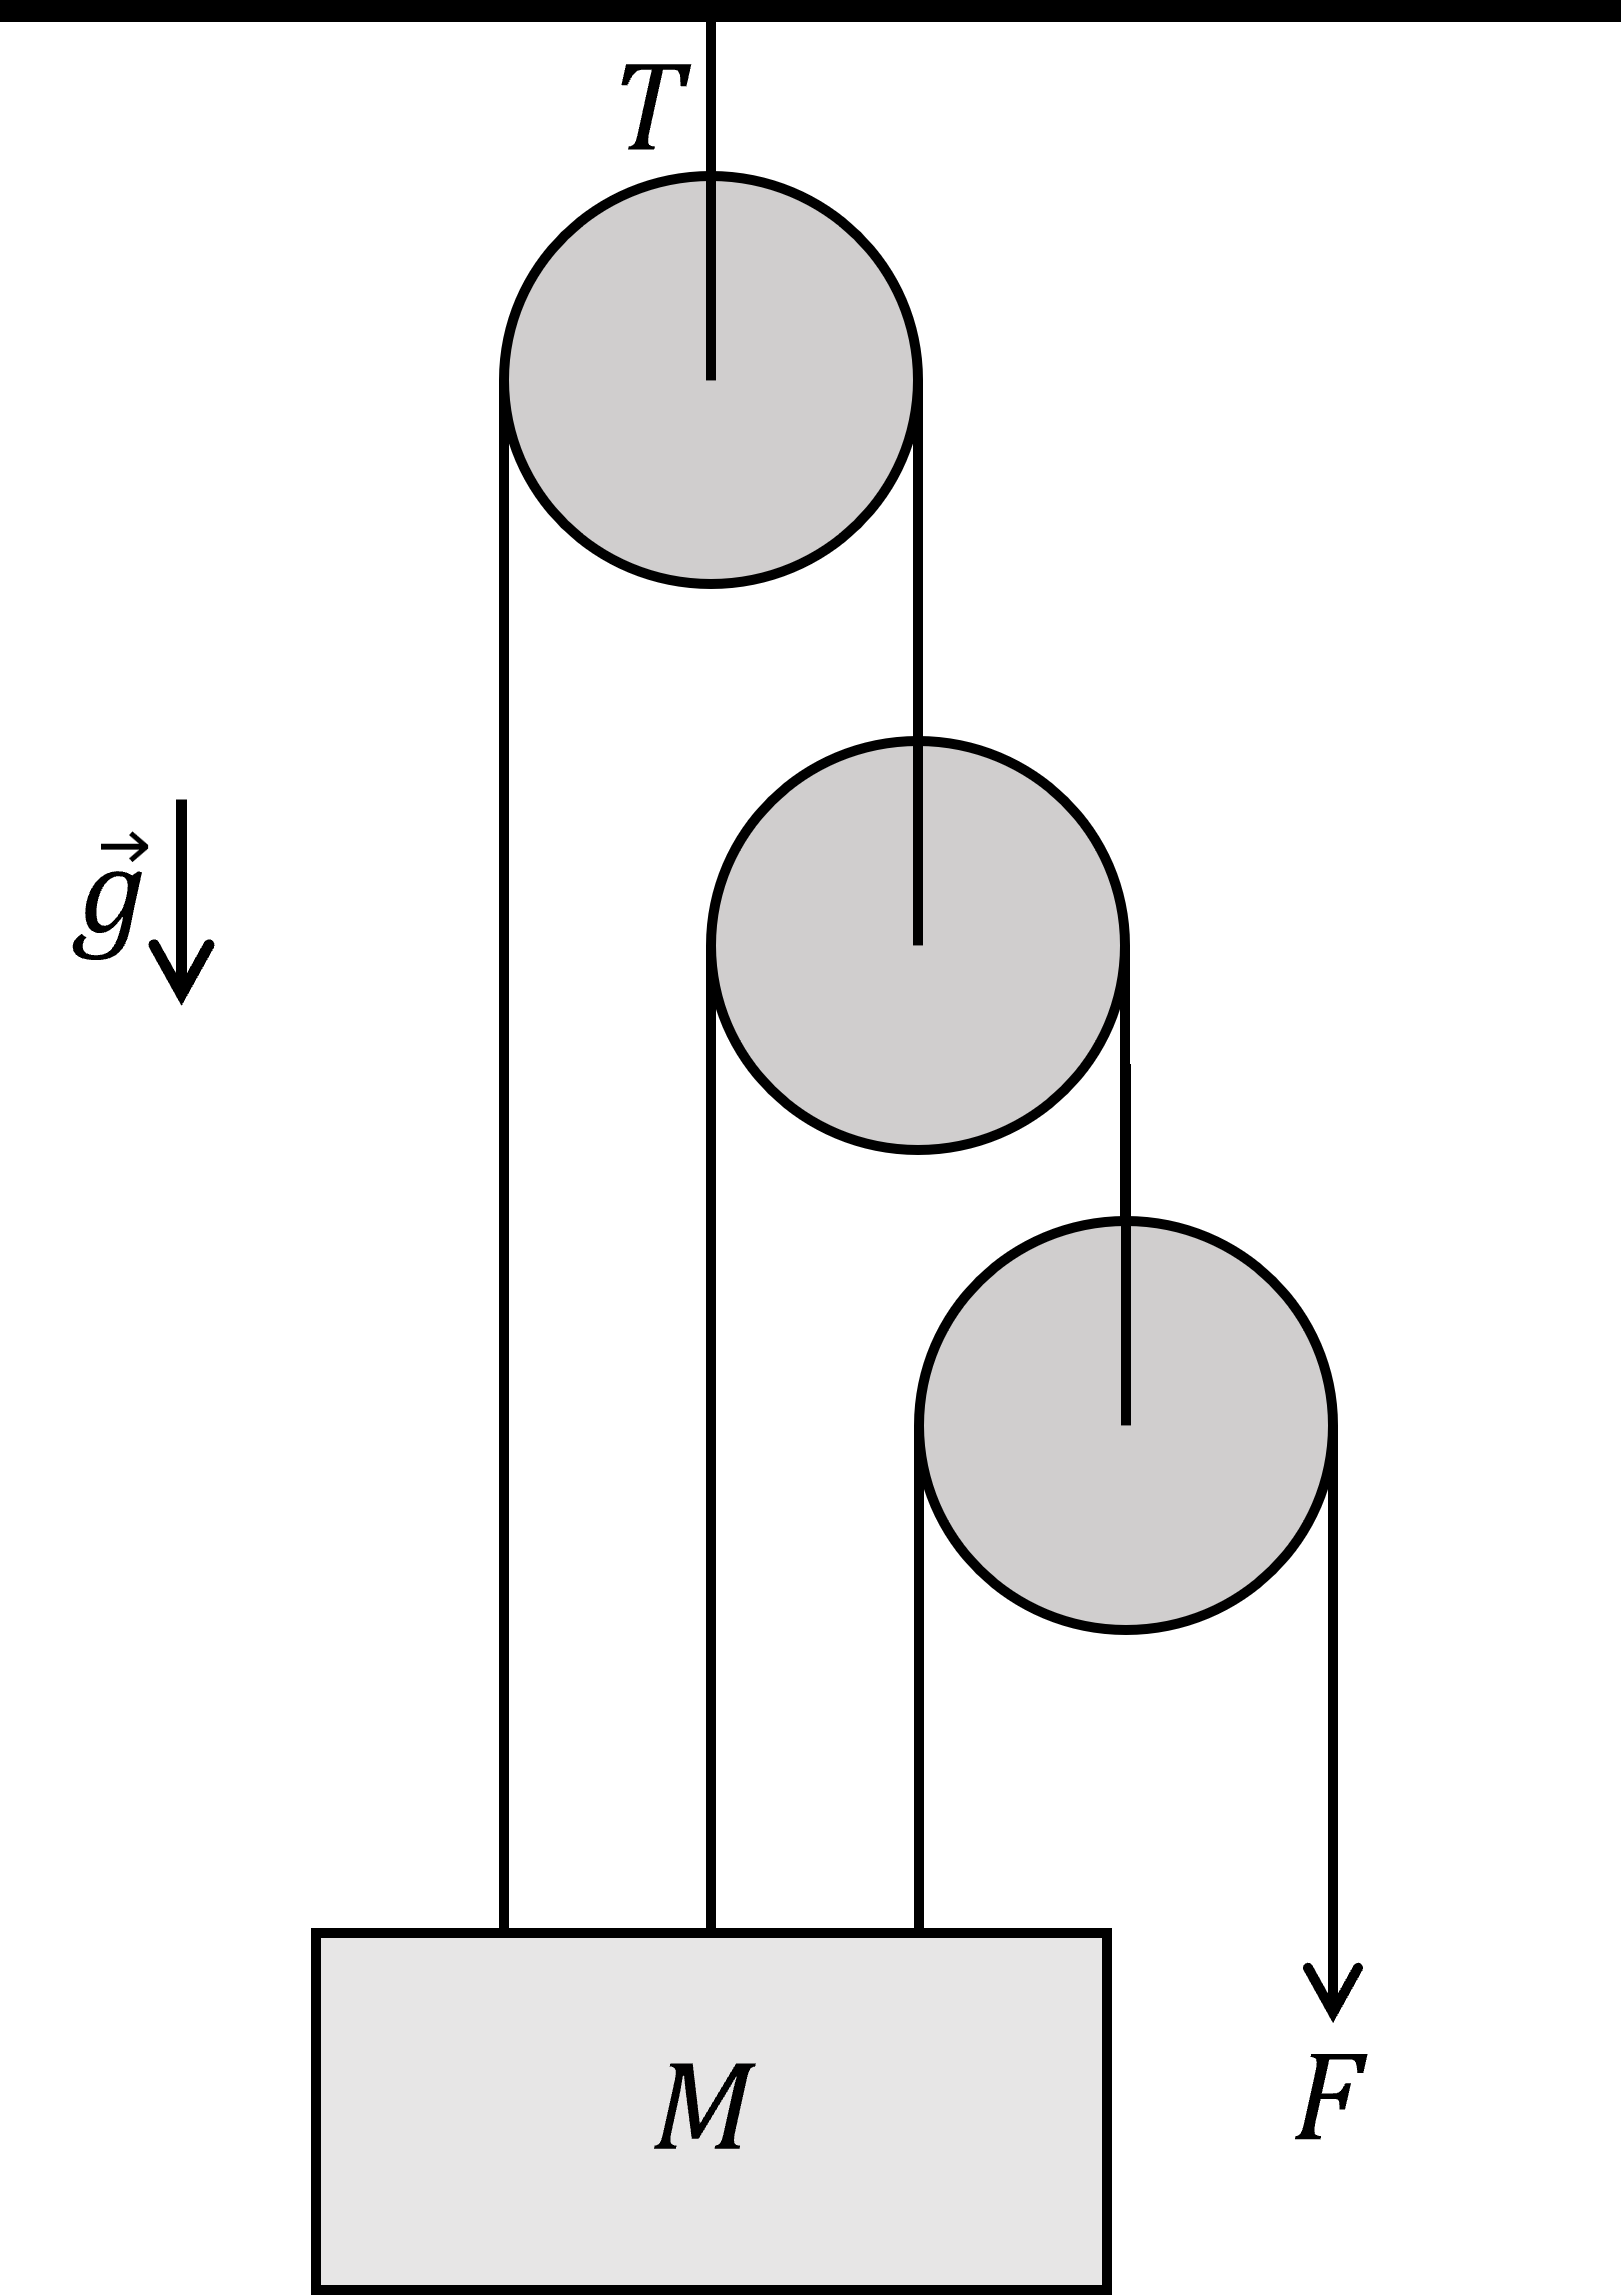
\includegraphics[width=0.4\linewidth]{2022-2/Imagenes/Taller6/polea1.png}
                \caption{P1a}
            \end{subfigure}
            \hspace{2em}
            \begin{subfigure}[t]{0.4\linewidth}
                \centering
                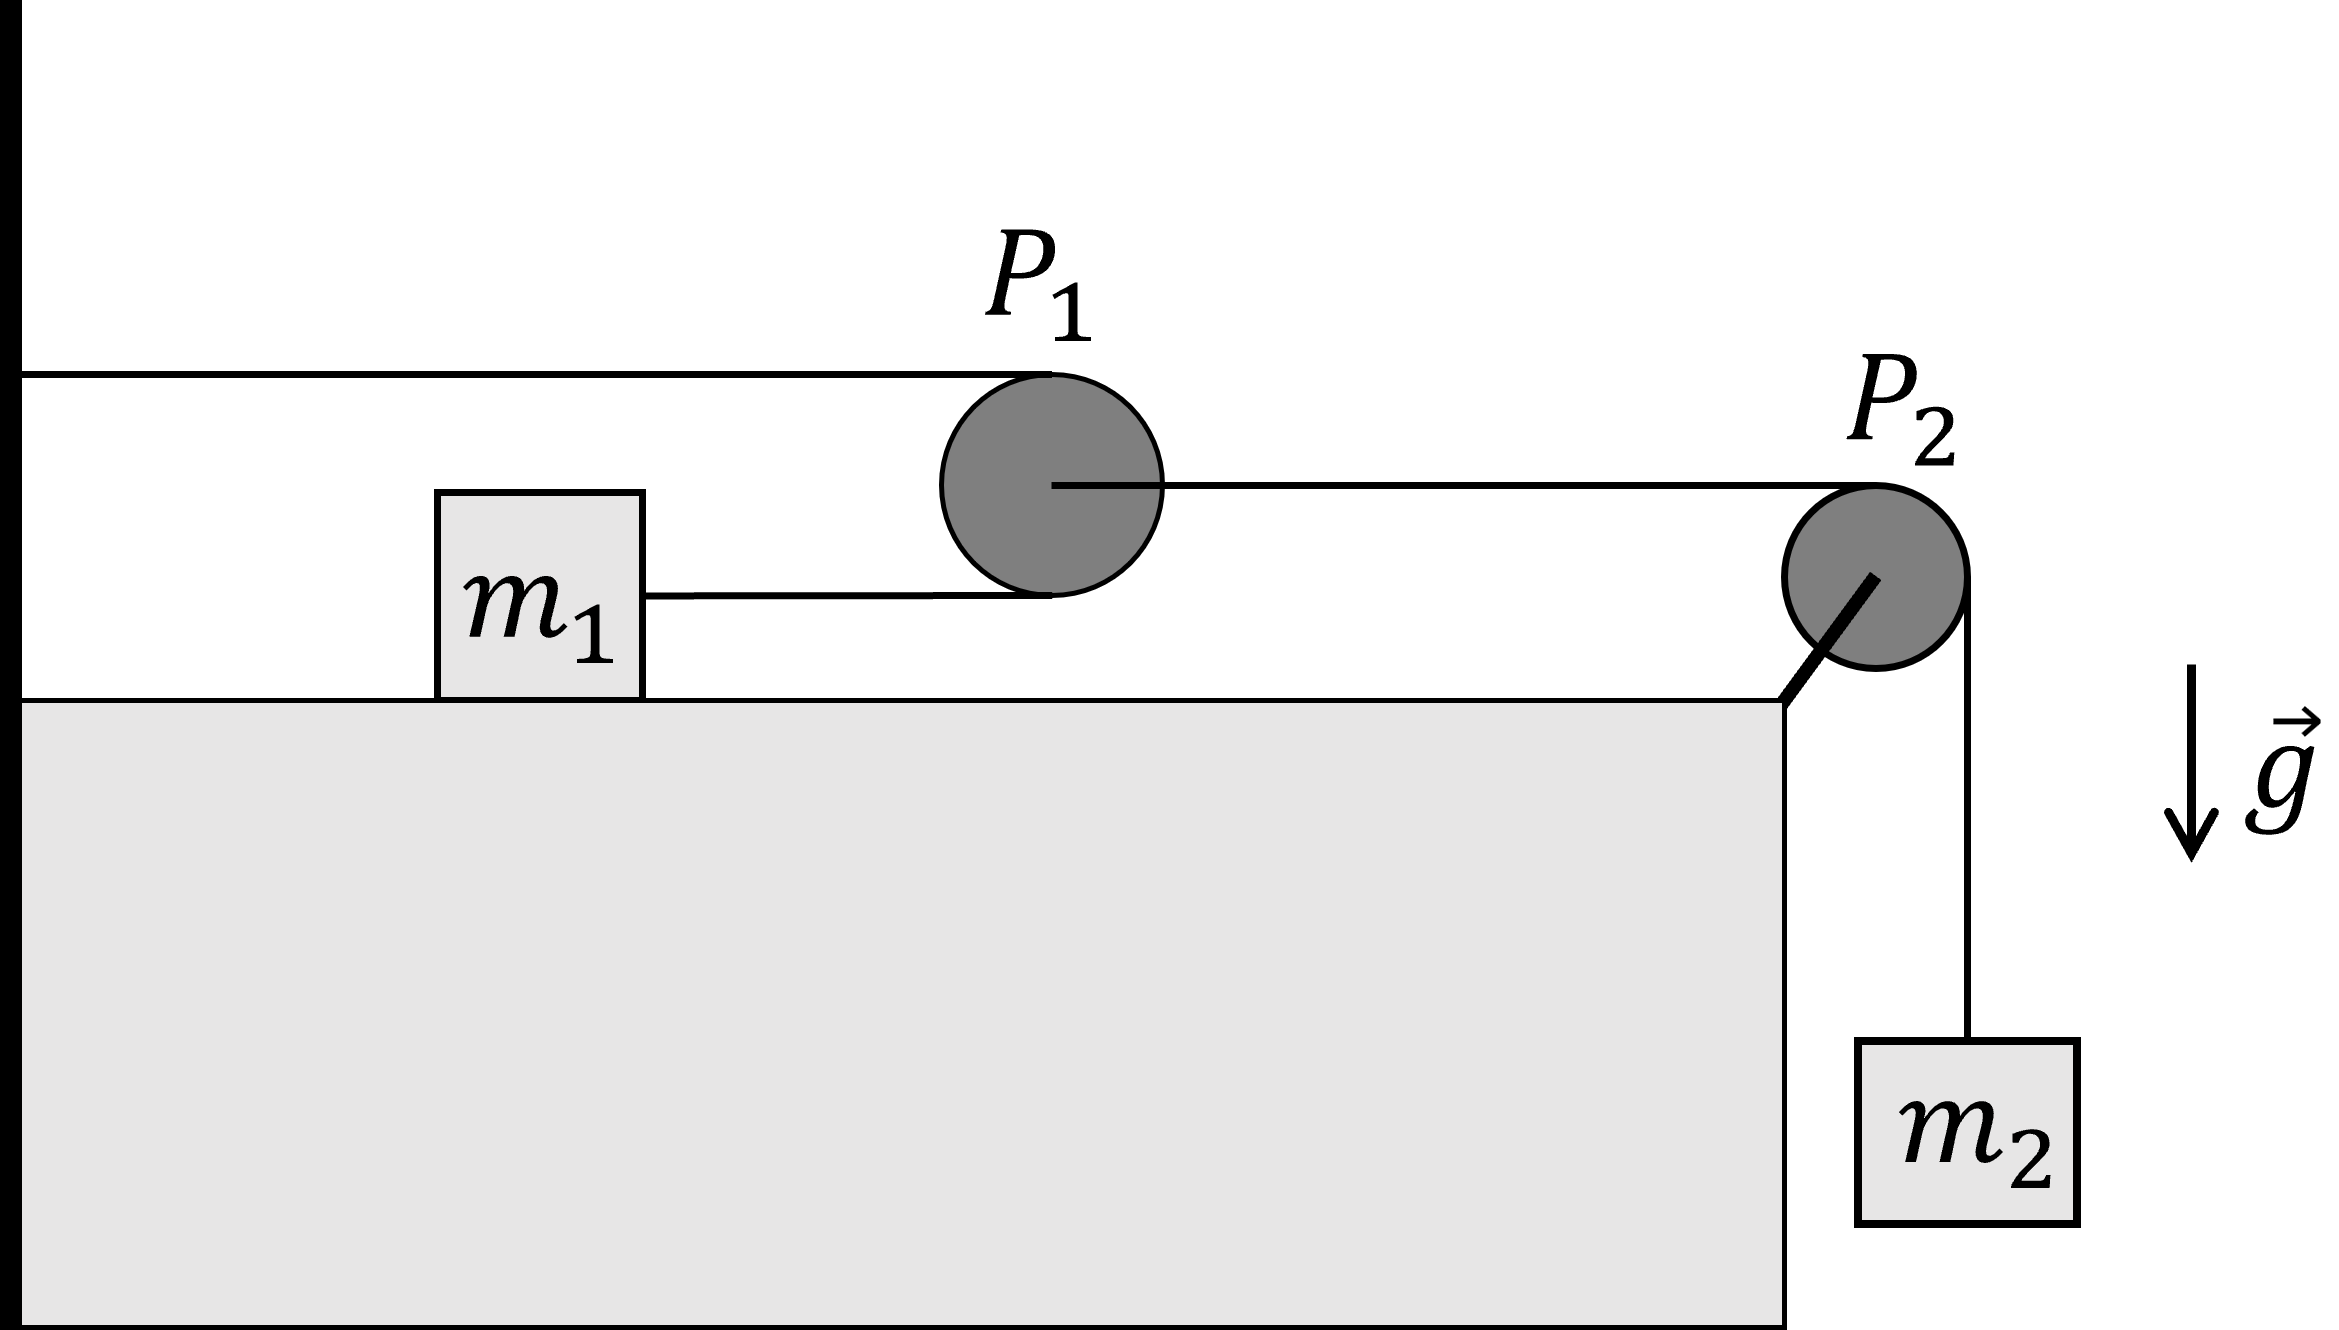
\includegraphics[width=0.8\linewidth]{2022-2/Imagenes/Taller6/polea2.png}
                \caption{P1b}
            \end{subfigure}
        \end{figure}
\end{enumerate}

\item \textbf{(Power Peralte)} Los \href{https://youtu.be/YX2MRz2vF7o?t=123}{\textbf{$Power \; Peralta$}} van derrapando en moto por la rotonda Grecia camino a su show en \href{https://www.youtube.com/watch?v=jof4a4U6aGA}{\textbf{Cunco City}}. La rotonda está peraltada de modo que ellos, desplazándose a una rapidez $v$, pueden tomar la curva de $R$, incluso si existe una capa de hielo equivalente a un coeficiente de fricción aproximadamente cero. A partir de esto, determinar: 

\begin{enumerate}
    \item El ángulo de inclinación del peralte $\theta$.
    
    \item Asumiendo que existe roce, el intervalo de velocidades a que los bailarines pueden tomar esta curva sin patinar si los coeficientes de roce estático y cinemático, entre la carretera y las ruedas, son $\mu_e$ y $\mu_c$ respectivamente.
\end{enumerate}

    \begin{figure}[H]
        \centering
        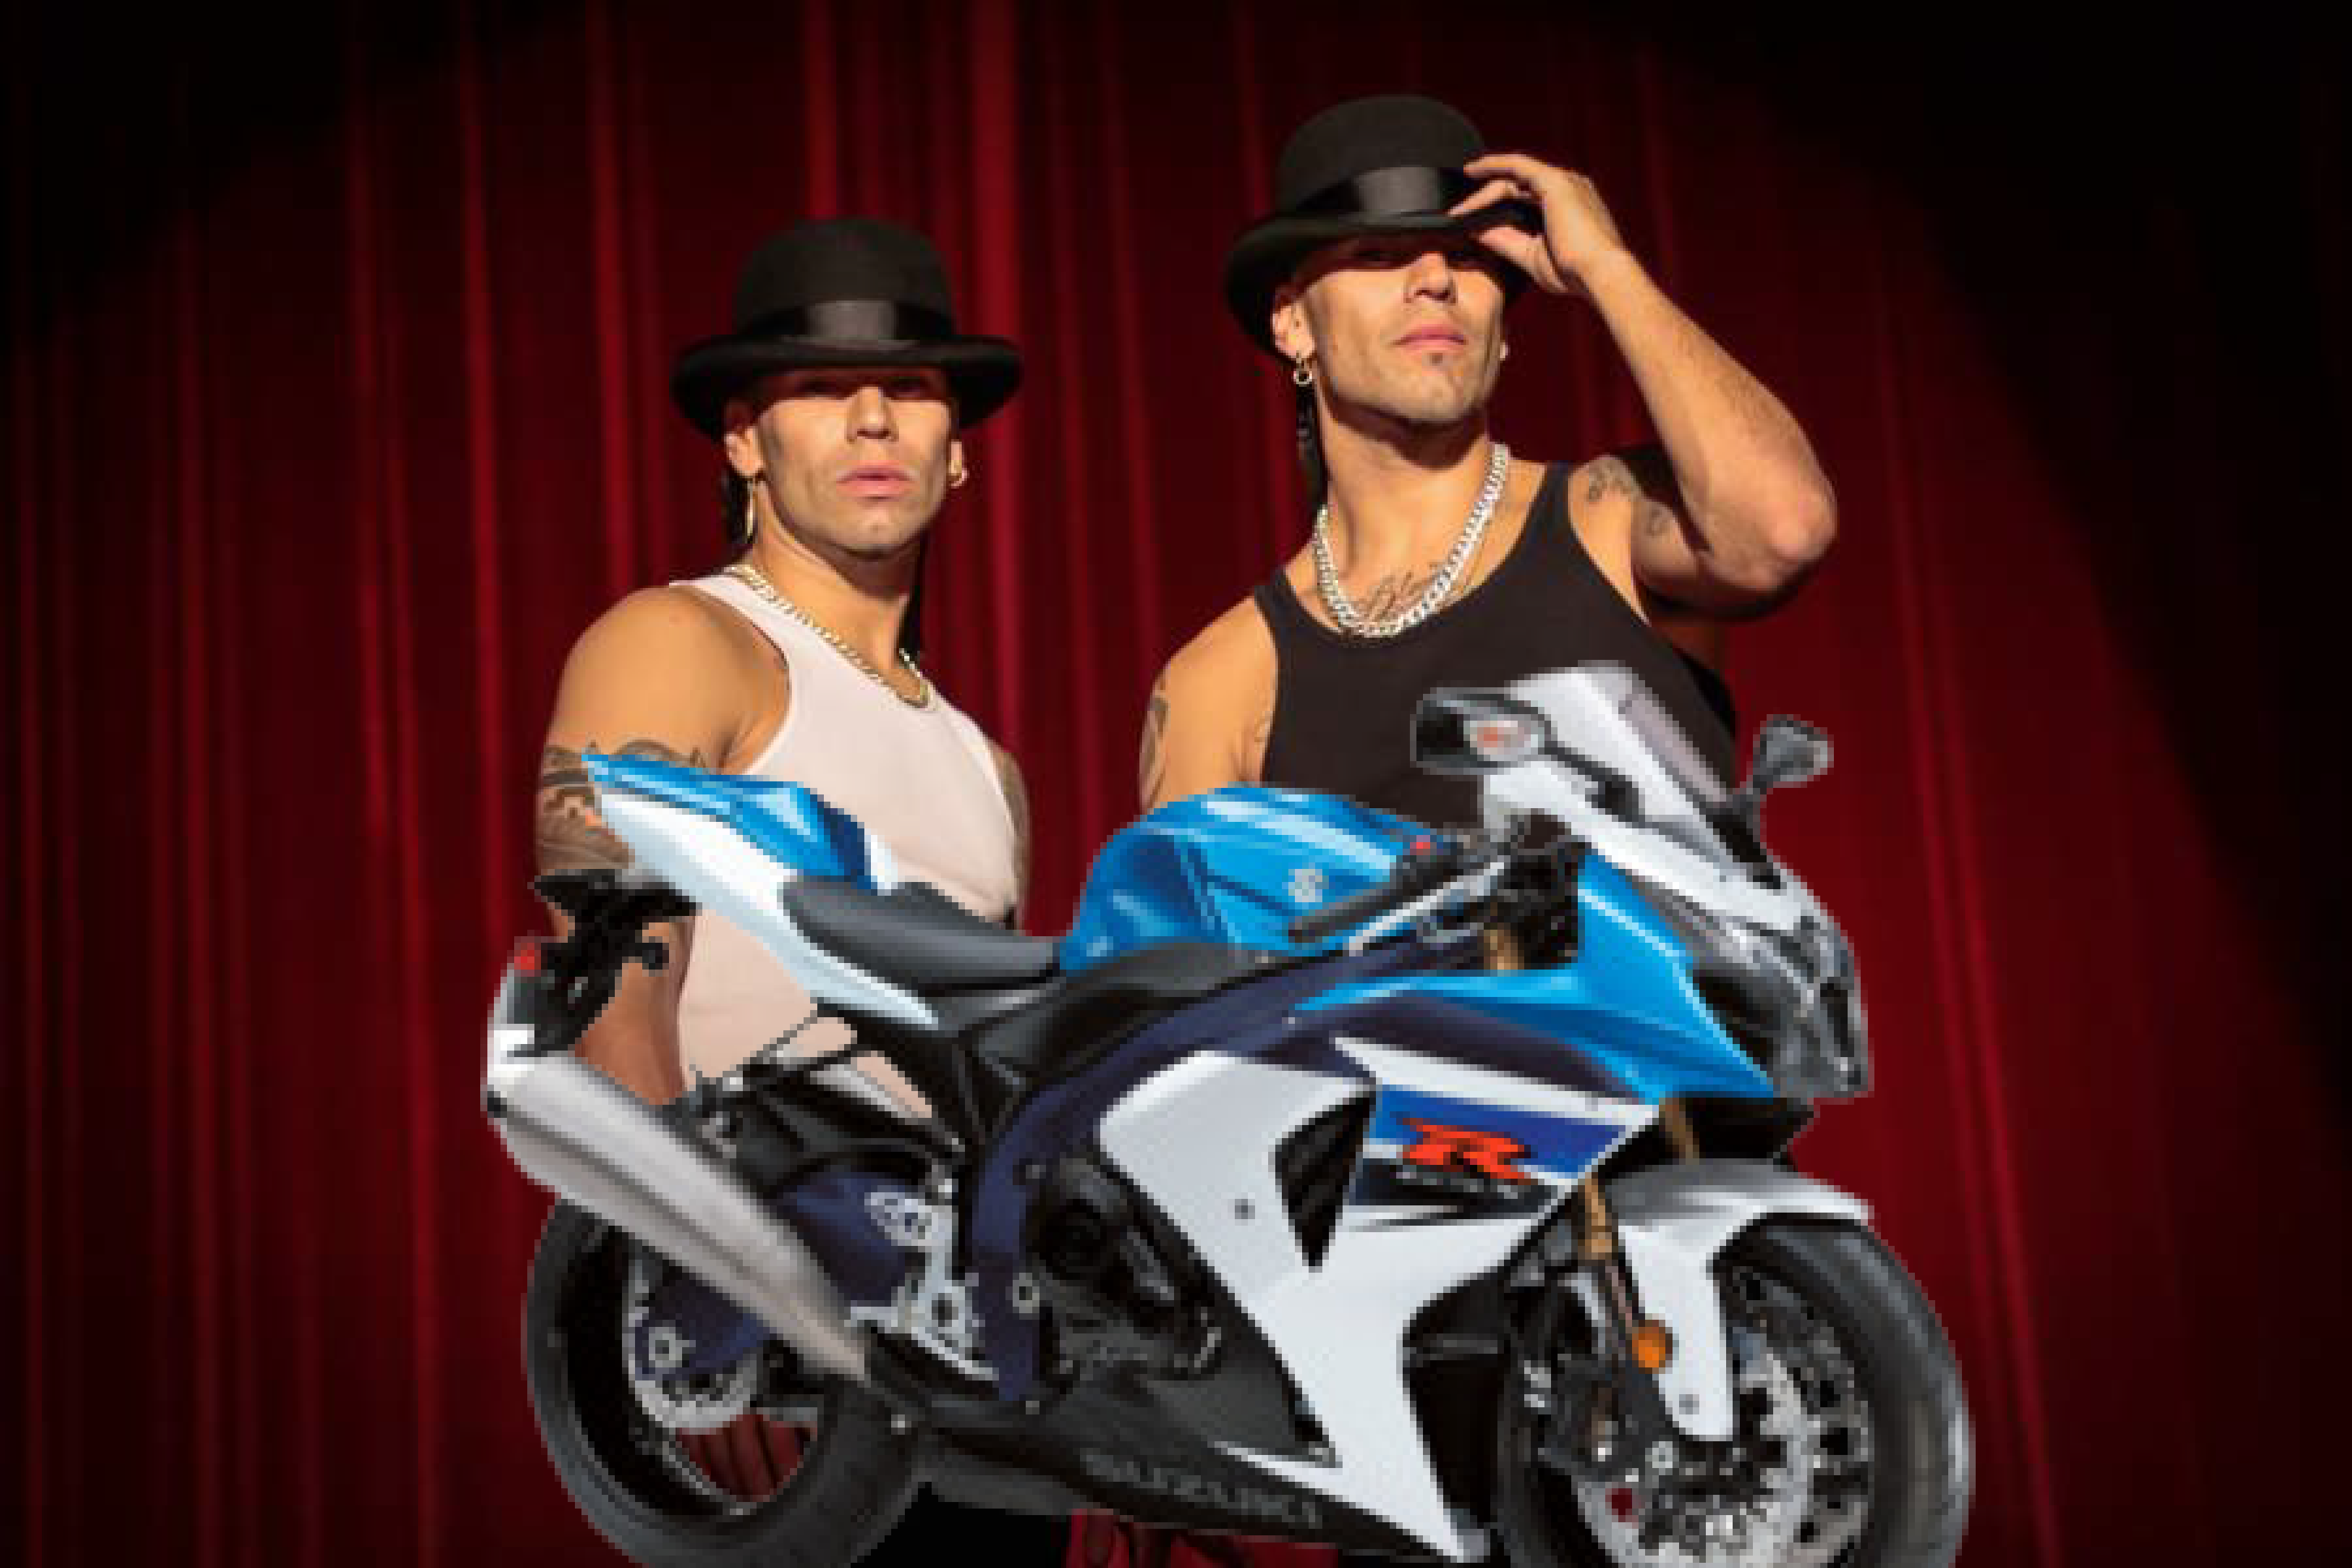
\includegraphics[width=0.39\linewidth]{2022-2/Imagenes/Taller6/PowerPeralte.png}
        \hspace{2em}
        \includesvg[width=0.39\linewidth]{../Imagenes/Taller6/p2.svg}  % le pasé el svg jeje

        \caption{P2 - Los Power Peralte}
    \end{figure} 




% Para imágenes vectoriales -> el texto tiene que estar en LaTeX
% \begin{figure}[htbp]
%   \centering
%   \svgpath{../Imagenes/ejercicios}  -> .. irse pa'trás 
%   \includesvg{ej5.svg}
% \end{figure}

\end{enumerate}
\end{document}
